% THIS DOCUMENT IS TAILORED TO REQUIREMENTS FOR SCIENTIFIC COMPUTING.  IT SHOULDN'T
% BE USED FOR NON-SCIENTIFIC COMPUTING PROJECTS
\documentclass[12pt]{article}

\usepackage{amsmath, mathtools}
\usepackage{amsfonts}
\usepackage{amssymb}
\usepackage{graphicx}
\usepackage{colortbl}
\usepackage{xr}
\usepackage{hyperref}
\usepackage{longtable}
\usepackage{xfrac}
\usepackage{tabularx}
\usepackage{float}
\usepackage{siunitx}
\usepackage{booktabs}
\usepackage{caption}
\usepackage{pdflscape}
\usepackage{afterpage}


\usepackage[round]{natbib}

%\usepackage{refcheck}

\hypersetup{
    bookmarks=true,         % show bookmarks bar?
      colorlinks=true,       % false: boxed links; true: colored links
    linkcolor=red,          % color of internal links (change box color with linkbordercolor)
    citecolor=green,        % color of links to bibliography
    filecolor=magenta,      % color of file links
    urlcolor=cyan           % color of external links
}

%% Comments

\usepackage{color}

\newif\ifcomments\commentstrue %displays comments
%\newif\ifcomments\commentsfalse %so that comments do not display

\ifcomments
\newcommand{\authornote}[3]{\textcolor{#1}{[#3 ---#2]}}
\newcommand{\todo}[1]{\textcolor{red}{[TODO: #1]}}
\else
\newcommand{\authornote}[3]{}
\newcommand{\todo}[1]{}
\fi

\newcommand{\wss}[1]{\authornote{blue}{SS}{#1}} 
\newcommand{\plt}[1]{\authornote{magenta}{TPLT}{#1}} %For explanation of the template
\newcommand{\an}[1]{\authornote{cyan}{Author}{#1}}

%% Common Parts

\newcommand{\progname}{ProgName} % PUT YOUR PROGRAM NAME HERE
\newcommand{\authname}{Team \#, Team Name
\\ Student 1 name
\\ Student 2 name
\\ Student 3 name
\\ Student 4 name} % AUTHOR NAMES                  

\usepackage{hyperref}
    \hypersetup{colorlinks=true, linkcolor=blue, citecolor=blue, filecolor=blue,
                urlcolor=blue, unicode=false}
    \urlstyle{same}
                                


% For easy change of table widths
\newcommand{\colZwidth}{1.0\textwidth}
\newcommand{\colAwidth}{0.13\textwidth}
\newcommand{\colBwidth}{0.82\textwidth}
\newcommand{\colCwidth}{0.1\textwidth}
\newcommand{\colDwidth}{0.05\textwidth}
\newcommand{\colEwidth}{0.8\textwidth}
\newcommand{\colFwidth}{0.17\textwidth}
\newcommand{\colGwidth}{0.5\textwidth}
\newcommand{\colHwidth}{0.28\textwidth}

% Used so that cross-references have a meaningful prefix
\newcounter{defnum} %Definition Number
\newcommand{\dthedefnum}{GD\thedefnum}
\newcommand{\dref}[1]{GD\ref{#1}}
\newcounter{datadefnum} %Datadefinition Number
\newcommand{\ddthedatadefnum}{DD\thedatadefnum}
\newcommand{\ddref}[1]{DD\ref{#1}}
\newcounter{theorynum} %Theory Number
\newcommand{\tthetheorynum}{TM\thetheorynum}
\newcommand{\tref}[1]{TM\ref{#1}}
\newcounter{tablenum} %Table Number
\newcommand{\tbthetablenum}{TB\thetablenum}
\newcommand{\tbref}[1]{TB\ref{#1}}
\newcounter{assumpnum} %Assumption Number
\newcommand{\atheassumpnum}{A\theassumpnum}
\newcommand{\aref}[1]{A\ref{#1}}
\newcounter{goalnum} %Goal Number
\newcommand{\gthegoalnum}{GS\thegoalnum}
\newcommand{\gsref}[1]{GS\ref{#1}}
\newcounter{instnum} %Instance Number
\newcommand{\itheinstnum}{IM\theinstnum}
\newcommand{\iref}[1]{IM\ref{#1}}
\newcounter{reqnum} %Requirement Number
\newcommand{\rthereqnum}{R\thereqnum}
\newcommand{\rref}[1]{R\ref{#1}}
\newcounter{nfrnum} %NFR Number
\newcommand{\rthenfrnum}{NFR\thenfrnum}
\newcommand{\nfrref}[1]{NFR\ref{#1}}
\newcounter{lcnum} %Likely change number
\newcommand{\lthelcnum}{LC\thelcnum}
\newcommand{\lcref}[1]{LC\ref{#1}}

\usepackage{fullpage}

\newcommand{\deftheory}[9][Not Applicable]
{
\newpage
\noindent \rule{\textwidth}{0.5mm}

\paragraph{RefName: } \textbf{#2} \phantomsection 
\label{#2}

\paragraph{Label:} #3

\noindent \rule{\textwidth}{0.5mm}

\paragraph{Equation:}

#4

\paragraph{Description:}

#5

\paragraph{Notes:}

#6

\paragraph{Source:}

#7

\paragraph{Ref.\ By:}

#8

\paragraph{Preconditions for \hyperref[#2]{#2}:}
\label{#2_precond}

#9

\paragraph{Derivation for \hyperref[#2]{#2}:}
\label{#2_deriv}

#1

\noindent \rule{\textwidth}{0.5mm}

}

\begin{document}

\title{Software Requirements Specification for \progname: RapidCare}
\author{\authname}
\date{\today}
	
\maketitle

~\newpage

\pagenumbering{roman}

\tableofcontents

~\newpage

\section*{Revision History}

\begin{tabularx}{\textwidth}{p{3cm}p{2cm}X}
\toprule {\bf Date} & {\bf Version} & {\bf Notes}\\
\midrule
Date 1 & 1.0 & Notes\\
Date 2 & 1.1 & Notes\\
\bottomrule
\end{tabularx}

\newpage

\pagenumbering{arabic}


\section{Introduction}

\subsection{Purpose of Document}

  The purpose of this document is to provide a comprehensive description of the requirements for a software application that aims to streamline the healthcare documentation process aimed to be run as a web application. This document will be used in as a contract in a sense between the team and the client who intends to use this application. This document will allow for an in-depth description of the software's functionality, performance, and other non-functional requirements. Additionally, it will outline common use-cases under which the software will be used. This will in turn provide a direction to the developers such that they will be empowered to creating the right product as this document will contain various stakeholders' requirements.\\

  Along with development direction, this document will be a direct reference for all of the stakeholders to understand the product's scope, functionality, and limitations. Additionally, this document will be a method of communication between the developers and stakeholders (domain experts, client, etc.) to ensure that the developers will be building the right product. This will ensure a feedback loop is established to allow for the development of a product that will satisfy the needs of the stakeholders and if project needs change it will be relayed through this document.


\subsection{Characteristics of Intended Reader} \label{sec_IntendedReader} 

The intended readers of this SRS document include project managers, software developers, testing engineers, and stakeholders directly involved in the design and implementation of the software system. Project managers and testing engineers would be directly involved in the development and testing process. They would generally have an education in computer science along with experience in software design, web or mobile development, and software testing. Project managers generally have experience in managing software projects and knowledge of software development processes. Stakeholders like doctors and nursing staff would have domain knowledge and could provide insights to understand the clinical workflow and documentation process. 

\subsection{Scope of Requirements} 


\subsubsection{Context Overall Objective}
Ontario is facing an extreme shortage of family doctors, with the number of
patients without one jumping by 600,000 to 2.5 million which is a growing
number [1]. This situation is only to get worse as predicted by the Ontario
Medical Association [2]. As a result, people find themselves going to the ER with
coughs and colds and flooding the ER causing massive wait times which ends in
patients even resulting in leaving without being seen [3]. A massive part of the
wait time is due to the overhead of documentation tasks. Doctors, healthcare
professionals, and support staff find themselves spending most of their time on
documentation which overall slows the pipeline of patients tremendously.

\subsubsection{Expected Benefits}
The expected benefits of this project are as follows:
\begin{itemize}
  \item Reduced documentation overhead time
  \item Increased patient throughput
  \item Improved patient care
  \item Increased doctor and healthcare professional satisfaction
\end{itemize}

Much like how copilot is a tool for programmers, the aim is to create a tool for healthcare professionals to help with documentation such that the number of patient processed per day can be increased, and the focus of doctors and nurses can be shifted from documentation to patient care. 

\subsubsection{Goals}
The goals for this project are as follows:
\begin{table}[H]
    \centering
    \begin{tabular}{p{4cm} p{4cm} p{4cm}}
        \toprule
        \textbf{Goal} & \textbf{Definition} & \textbf{Rationale} \\
        \midrule
        G1: Use voice to fill in medical documentation (charts, files, etc.) & The app will record conversations and automatically turn them into medical notes and charts. & This will save doctors time by automating paperwork, letting them focus more on patients. \\
        \midrule
        G2: Reduce documentation overhead time.  & Through tracking the whole patient journey in the app, we look to reduce the overhead of triaging, clinical documentation, and other registrations.  & This helps hospital healthcare professionals focus on care and lowers the time taken through registration for hospital staff. \\ 
        \midrule
        G3: Compliant with data security standards.  & Patient data will flow through the app therefore the app must abide by privacy laws and privacy standards. & This will give healthcare organizations confidence in the application and will give patients peace of mind that their information is safe. \\
        \midrule 
        G4: Ease of integration with the existing hospital environment. & We want the solution to be portable such that it can be implemented in existing hospital and clinic ecosystems.  & Portability will ensure that hospitals and clinics won’t have to upgrade their existing hardware to use the application. \\
        \midrule 
        G5: Ease of use. & The app will be designed so that healthcare professionals of all skill levels can use it without any difficulty. & A simple, intuitive interface ensures users can quickly learn and use the app, allowing them to spend more time on patient care rather than managing the system. \\
        \bottomrule
    \end{tabular}
\end{table}

\subsubsection{Stretch Goals}
The stretch goals for this project are as follows:
\begin{table}[H]
    \centering
    \begin{tabular}{p{4cm} p{4cm} p{4cm}}
        \toprule
        \textbf{Goal} & \textbf{Definition} & \textbf{Rationale} \\
        \midrule
        STG1: Automated medicine suggestions. & Based on diagnosis and patient data provide medicine suggestions. & This will help doctors fill out their charts faster. \\ % Row 1
        \midrule
        STG2: Automated diagnosis suggestions.  & Use AI to suggest possible diagnoses based on what the doctor and patient discuss.  & This will help doctors make faster, more accurate diagnoses, especially in tricky cases.\\ 
        \midrule
        STG3: Machine learning for triage.  & Use machine learning to prioritize patients based on the severity of their condition. & This ensures the most critical patients get treated first, improving care in emergencies. \\
        \midrule 
        STG4: Multi-language support. & Let doctors and patients use the app in different languages.  & This makes the app useful for a wider range of people, especially in diverse hospitals. \\
        \bottomrule
    \end{tabular}
\end{table}

% \begin{itemize}
% \item[GS\refstepcounter{goalnum}\thegoalnum \label{G_meaningfulLabel}:] \plt{One
%     sentence description of the goal.  There may be more than one.  Each Goal
%     should have a meaningful label.}
% \end{itemize}

% References at the end of the document

\subsection{Organization of Document}
The organization of this document is as follows:
\begin{itemize}
  \item \textbf{System Description}\\
  This section will provide an overview of the system, its functionality, the characteristics of the users, and the constraints of the system.
  \item \textbf{Requirements}\\
  This section will outline the functional and non-functional requirements. Additionally, it will provide a rationale for all of the requirements.
  \item \textbf{Likely Changes}\\
  This section will outline the likely changes that may occur in the future.
  \item \textbf{Unlikely Changes}\\
  This section will outline the unlikely changes that may occur in the future.
  \item \textbf{References}\\
  This section will provide a list of references used in the document.

\end{itemize}

~\newpage

\section{System Description}

\subsection{Definitions, Acronyms, and Abbreviations}

\begin{tabular}{l l} 
  \toprule    
  \textbf{symbol} & \textbf{description}\\
  \midrule 
  A & Assumption\\
  G & Goal Statement\\
  LC & Likely Change\\
  R & Requirement\\
  SRS & Software Requirements Specification\\
  EHR & Electronic Healthcare record\\
  STG & Stretch Goals\\
  \bottomrule
\end{tabular}\\

The following is the glossary for this document:

\textbf{System} -- When referring to a system the document refers to the intended solution/product.


\textbf{User} -- When referring to a user the document refers to a person who will use the product.


\subsection{System overview}

This product has been conceived by the group members based on elicitation. Through interviews and discussion the problem of documentation overhead was found. This is the problem to be solved for the capstone course SFWRENG 4G06.\\

Through this project we aim to develop a solution that will address key niche problems through customizability and add features of critical need that do not already exist in existing solutions. This will allow healthcare networks to centralize the data of their hospitals and increase the staff productivity.

\subsection{System Functionality}

This section outlines the core functionalities and characteristics of the proposed system:

\begin{itemize}
  \item \textbf{Patient Documentation} -- The system should facilitate efficient and streamlined patient documentation throughout the EHR documentation process. This includes storing patient data, clinical notes, treatment plans, and patient history in a secure mamnner.
  
  \item \textbf{Voice Recording and Transcription} -- The system should be able to record conversations between healthcare professionals and patients which will be transcribed to fill out charts and patient profiles efficiently.
  
  \item \textbf{Real-time Data Access} –- The users must have real-time access to patient data and documentation enabling them to make informed decisions quickly and efficiently.
  
  \item \textbf{Automated Medicine Suggestions} –- The system should be able to provide automated medicine suggestions based on the transcribed data which will help users to fill out the charts faster and make informed treatment decisions.
  
  \item \textbf{Automated Diagnosis Suggestions} -- The system should be able to suggest possible diagnoses based on transcribed data which will help users to make faster and more accurate diagnoses.
  
  \item \textbf{User Authentication} -- The system must provide secure user authentication methods to ensure that only authorized personnel can access sensitive patient information.
  
  \item \textbf{Data Privacy} -- The system must store all patient data in a secure manner to avoid any data privacy and regulatory concerns.
  
\end{itemize}


\subsection{User Characteristics} \label{SecUserCharacteristics}

The intended users of this product are healthcare professionals, specifically those involved in patient documentation, including doctors, nurses, and other clinical administrative staff. 

The following are the user characteristics associated with the intended users:

\textbf{Education Level} -- All users are expected to have a minimum of a college diploma and basic reading, writing, and speaking skills. The education level of the intended users will vary based on their role, generally a bachelor’s degree or college diploma in nursing, medicine, or other healthcare fields. 

\textbf{Experience} -- All users will be expected to have basic familiarity with EHR systems or similar applications. This experience will depend on their roles ranging from entry-level positions to experienced professionals. 

\textbf{Technical Expertise} -- The users should have basic technical skills to use EHR systems and other healthcare software applications. In addition to this, the users should have familiarity with data entry processes and analytics interpretation.

\textbf{Accessibility Considerations} -- It is anticipated that some users may have accessibility issues. The user interface should be designed for ease of navigation, incorporating various accessibility features.

Specific requirements must be specified to accommodate users with varying technical expertise and diverse educational backgrounds. This will ensure the application is usable by all healthcare staff, regardless of their abilities.


\subsection{System Constraints}

The following constraints will guide the system design and implementation:

\begin{itemize} 
  \item \textbf{System Compatibility} -- The system must be compatible with existing EHR systems for seamless integration and data exchange.

  \item \textbf{Compliance with Regulatory Standards} -- The system must adhere to healthcare regulations ensuring the confidentiality and security of patient data.

  \item \textbf{User Accessibility} -- The system must meet established accessibility standards to ensure usability for all healthcare staff, including those with disabilities.

  \item \textbf{Cost and Time} -- The system must be developed within the imposed budget and time restrictions.

\end{itemize}

\subsubsection{Assumptions and Dependencies} \label{sec_assumpt}

\begin{itemize}
  \item\textbf{Reliable Internet Connection} -- We are assuming that user has a reliable internet connection throughout the patient’s visit as it is essential for authentication to the app, real-time interaction with it, running updates and saving the document to the patient’s profile.
  \item\textbf{Sufficient Hardware Accessories} -- We are assuming that the hospital staff has enough hardware devices such as monitors, iPads etc. to access the software.
  \item\textbf{Patient’s Comfort} -- We also assume that patients are comfortable using this software, ensuring that their information will be kept private and secure on their profile.
\end{itemize}

\subsubsection{Usage Scanerios}

Here are the use-case scenarios for this software--

\begin{itemize}
  \item\textbf{UC1 Recording Clinical Notes} --
  \begin{itemize}
    \item Healthcare professional accesses patient’s profile.
    \item Healthcare professional selects dictate button.
    \item Healthcare professional takes clinical notes.
  \end{itemize}
  \item\textbf{UC2 Generate Diagnostic Suggestions} --
  \begin{itemize}
    \item Healthcare professional will review the notes.
    \item App checks symptoms and suggests potential diagnosis and treatment options.
    \item Doctor verifies the options.
    \item Doctor decides to accept or reject.
  \end{itemize}
\end{itemize}

\textbf{Usage Scenario 1 : Documenting a Patient Consultation}

\begin{itemize}
  \item\textbf{Use Case} -- UC1
  \item\textbf{Primary Actor} -- Healthcare professional (such as a medical doctor or a nurse)
  \item\textbf{Precondition} -- The healthcare professional has authentication to log in the system and patient’s profile is opened. The basic information such as name, contact information and illness history are already filled.
  \item\textbf{Trigger} -- The healthcare professional will press the record button.
  \item\textbf{Main Success Scenario} --
  \begin{itemize}
    \item The doctor will press the button for dictation tool.
    \item The software will convert audio to text in real-time and produce text.
    \item The user will press complete button.
    \item  The doctor will review the notes produced.
    \item The doctor will press the submit button if everything is ok.
  \end{itemize}
  \item\textbf{Secondary Success Scenario} --
  \begin{itemize}[label=6.\arabic*]
    \item If any mistake is found, the doctor will edit the notes manually.
    \item Doctor submits the final version of the notes.
  \end{itemize}
  \item\textbf{Success Postcondition} --
  \begin{itemize}
    \item The notes are saved in patient’s profile in a secure manner.
  \end{itemize}
\end{itemize}

\begin{figure}[h]
  \centering
  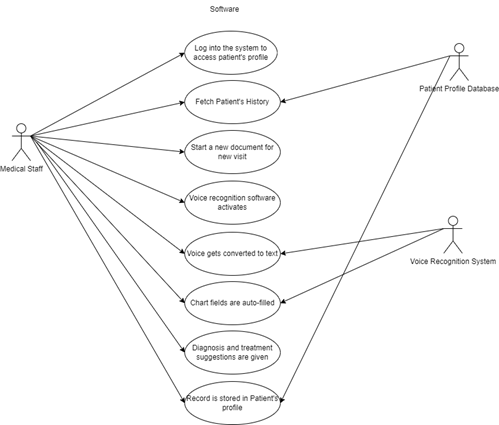
\includegraphics[width=0.8\textwidth]{use_case_diag.png}
  \caption{This is the use-case diagram for this project.}
  \label{fig:Use-Case Diagram}
\end{figure}

\begin{figure}[h]
  \centering
  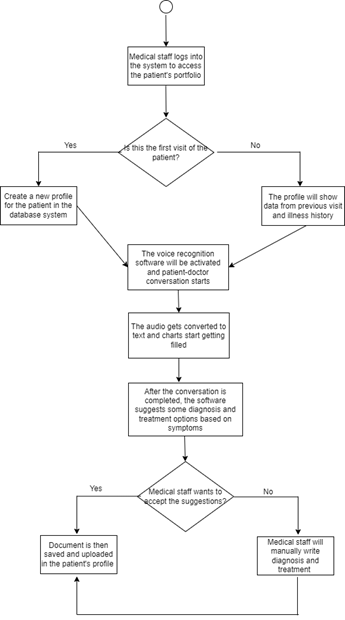
\includegraphics[width=0.8\textwidth]{activity_diag.png}
  \caption{This is the activity diagram for this project.}
  \label{fig:Activity Diagram}
\end{figure}

\subsubsection{Risks and Mitigation}

Looking at implementation details there are a few risks that come up, if these risks can be addressed or have a clearer roadmap that will make us more confident in the project. 

\begin{itemize}
  \item \textbf{Speech Input} -- A hospital or a clinic can be a loud place, in the event audio input is taken we need to ensure that it is clean and clear. This would mean essentially blocking outside noise. 
  \item \textbf{Visual Inputs} -- If any old charts need to be inputted into the patient journey having the ability to scan and transfer the information into the required format will be another risk. The document needs to be rid of noisy data.
  \item \textbf{Pre-Trained Models} -- To manipulate and use both inputs above we need to create a model to be accurate and provide accuracy when filling in charts. 
  \item \textbf{Data Privacy} -- This application will hold a lot of patient data so creating a store that is secure and making sure standard data security practice is applied is a must.
  \item \textbf{User Acceptance} -- This will require further elicitation from outside supervisors. We need to gather data on what critical needs of healthcare professionals such that critical features are present.
  \item \textbf{Technical Delay} -– Integration with Electronic Health record systems might cause some delays if there’s any technical issue or if the software faces compatibility issues. This will require sample testing to make sure that the software is compatible in the early stage of the development process.
  \item \textbf{Professional Verification} -– Misinterpretation of some words might lead to inaccurate records and wrong diagnosis. Therefore, it’s important for the doctor/nurse to verify the final version of the document and manually delete anything that was falsely recorded. 
\end{itemize}

~\newpage

\section{Requirements}

This section provides the functional requirements, the business tasks that the
software is expected to complete, and the nonfunctional requirements, the
qualities that the software is expected to exhibit.

\subsection{Functional Requirements}

\noindent \begin{itemize}

\item[R\refstepcounter{reqnum}\thereqnum \label{R_Inputs}:] \plt{Requirements
    for the inputs that are supplied by the user.  This information has to be
    explicit.}

\item[R\refstepcounter{reqnum}\thereqnum \label{R_OutputInputs}:] \plt{It isn't
    always required, but often echoing the inputs as part of the output is a
    good idea.}

\item[R\refstepcounter{reqnum}\thereqnum \label{R_Calculate}:] \plt{Calculation
    related requirements.}

\item[R\refstepcounter{reqnum}\thereqnum \label{R_VerifyOutput}:]
  \plt{Verification related requirements.}

\item[R\refstepcounter{reqnum}\thereqnum \label{R_Output}:] \plt{Output related
    requirements.}

\end{itemize}

\plt{Every IM should map to at least one requirement, but not every requirement
  has to map to a corresponding IM.}

\subsection{Non-functional Requirements}

\noindent \begin{itemize}

\item[NFR\refstepcounter{nfrnum}\thenfrnum \label{NFR_Performance}:] \textbf{Performance}  
    
    \textbf{Requirement:} The system shall process voice recordings and convert them into medical charts within 30 seconds of recording completion.  
  
    \textbf{Rationale:} Quick documentation is critical to streamline the patient journey and reduce healthcare professionals' workload.  
  
    \textbf{Fit Criterion:} The system will consistently generate completed documentation in under 30 seconds.  
  
    \textbf{Dependencies:} Dependent on the speech-to-text engine and cloud infrastructure.  
  
    \textbf{Normal Operation:} Under typical conditions, the system will handle up to 100 voice recordings per hour without performance degradation.  
  
    \textbf{Undesired Event Handling:} If the system takes longer than 30 seconds, an alert will be triggered, and the system will attempt to resolve delays by reducing background processes or scaling resources.

\item[NFR\refstepcounter{nfrnum}\thenfrnum \label{NFR_Reliability}:] \textbf{Reliability}  

    \textbf{Requirement:} The system shall have a 99.9\% uptime guarantee during operational hours (9 AM to 9 PM).  
  
    \textbf{Rationale:} Reliability is critical to ensure uninterrupted service for healthcare professionals, particularly in time-sensitive environments like emergency rooms.  
  
    \textbf{Fit Criterion:} System logs will confirm an uptime rate of 99.9\% over a 30-day period.  
  
    \textbf{Dependencies:} Cloud infrastructure, hosting services, and local hardware resilience.  
  
    \textbf{Undesired Event Handling:} If uptime falls below 99.9\%, an automated system will switch to backup servers within 10 seconds to ensure continuity of service.

\item[NFR\refstepcounter{nfrnum}\thenfrnum \label{NFR_Scalability}:] \textbf{Scalability}  

    \textbf{Requirement:} The system shall be able to scale to accommodate up to 500 simultaneous users without affecting performance.  
  
    \textbf{Rationale:} The system must support multiple healthcare providers across various locations, particularly during peak hours.  
  
    \textbf{Fit Criterion:} The system will maintain performance benchmarks (processing under 30 seconds) even when 500 users are active.  
  
    \textbf{Dependencies:} Cloud infrastructure for auto-scaling capabilities.  
  
    \textbf{Normal Operation:} The system will maintain user load without affecting response time.  
  
    \textbf{Undesired Event Handling:} In case of unexpected spikes in usage, the system will dynamically allocate additional cloud resources to manage the load without affecting current users.

\item[NFR\refstepcounter{nfrnum}\thenfrnum \label{NFR_Security}:] \textbf{Security}  

    \textbf{Requirement:} The system shall encrypt all patient data, both in transit and at rest, following HIPAA standards.  
  
    \textbf{Rationale:} Ensuring patient confidentiality and compliance with healthcare data regulations is essential.  
  
    \textbf{Fit Criterion:} Security audits will show 100\% compliance with HIPAA and encryption standards.  
  
    \textbf{Dependencies:} Encryption services and security protocols in the cloud infrastructure.  
  
    \textbf{Undesired Event Handling:} If a security breach is detected, the system will immediately log out all users, lock access to sensitive data, and alert system administrators.

\item[NFR\refstepcounter{nfrnum}\thenfrnum \label{NFR_Usability}:] \textbf{Usability}  

    \textbf{Requirement:} The system’s user interface shall be intuitive, allowing healthcare professionals to complete documentation with minimal training (less than 30 minutes of training).  
  
    \textbf{Rationale:} A user-friendly interface reduces learning time and increases adoption among healthcare providers.  
  
    \textbf{Fit Criterion:} Usability tests will show that 90\% of healthcare professionals can navigate the system with less than 30 minutes of instruction.  
  
    \textbf{Dependencies:} Usability design and feedback loops during development.  
  
    \textbf{Undesired Event Handling:} If users encounter usability issues, they can access live chat support integrated within the application.

\item[NFR\refstepcounter{nfrnum}\thenfrnum \label{NFR_Maintainability}:] \textbf{Maintainability}  

    \textbf{Requirement:} The system shall be updated with new features without causing downtime for more than 5 minutes.  
  
    \textbf{Rationale:} Frequent updates should not disrupt healthcare professionals during critical hours.  
  
    \textbf{Fit Criterion:} Release notes and system logs will show that updates occur with less than 5 minutes of downtime, or during non-operational hours.  
  
    \textbf{Dependencies:} Continuous integration and delivery pipelines.  
  
    \textbf{Undesired Event Handling:} In case of an update failure, the system will automatically revert to the last stable version.

\item[NFR\refstepcounter{nfrnum}\thenfrnum \label{NFR_Compatibility}:] \textbf{Compatibility}  

    \textbf{Requirement:} The system shall be compatible with major operating systems (Windows, macOS, and Linux) and dictation devices.  
  
    \textbf{Rationale:} Healthcare providers use a variety of platforms, and the system must be versatile to support their workflows.  
  
    \textbf{Fit Criterion:} Compatibility tests will show full functionality on all major operating systems and devices used for dictation.  
  
    \textbf{Dependencies:} Device drivers and OS compatibility libraries.  
  
    \textbf{Undesired Event Handling:} If a compatibility issue arises, the system will notify the user and suggest an alternative setup or device.

\item[NFR\refstepcounter{nfrnum}\thenfrnum \label{NFR_DataIntegrity}:] \textbf{Data Integrity}  

    \textbf{Requirement:} The system shall prevent duplicate or erroneous data entries when processing voice recordings.  
  
    \textbf{Rationale:} Data accuracy is critical in healthcare documentation, where errors could lead to incorrect treatment or diagnosis.  
  
    \textbf{Fit Criterion:} Data audits will show no more than 0.1\% duplication or errors in generated medical charts.  
  
    \textbf{Dependencies:} Data validation protocols and the speech-to-text engine.  
  
    \textbf{Undesired Event Handling:} In case of detected duplicates or errors, the system will automatically flag the entry for review and notify the healthcare professional.

\end{itemize}

\subsection{Rationale}

\plt{Provide a rationale for the decisions made in the documentation.  Rationale
should be provided for scope decisions, modelling decisions, assumptions and
typical values.}

\section{Likely Changes}    

\noindent \begin{itemize}

\item[LC\refstepcounter{lcnum}\thelcnum\label{LC_meaningfulLabel}:] \plt{Give
    the likely changes, with a reference to the related assumption (aref), as appropriate.}

\end{itemize}

\section{Unlikely Changes}    

\noindent \begin{itemize}

\item[LC\refstepcounter{lcnum}\thelcnum\label{LC_meaningfulLabel}:] \plt{Give
    the unlikely changes.  The design can assume that the changes listed will
    not occur.}

\end{itemize}

~\newpage

\section{References}

\newpage{}
\section*{Appendix --- Reflection}

\wss{Not required for CAS 741}

The information in this section will be used to evaluate the team members on the
graduate attribute of Lifelong Learning.  

The purpose of reflection questions is to give you a chance to assess your own
learning and that of your group as a whole, and to find ways to improve in the
future. Reflection is an important part of the learning process.  Reflection is
also an essential component of a successful software development process.  

Reflections are most interesting and useful when they're honest, even if the
stories they tell are imperfect. You will be marked based on your depth of
thought and analysis, and not based on the content of the reflections
themselves. Thus, for full marks we encourage you to answer openly and honestly
and to avoid simply writing ``what you think the evaluator wants to hear.''

Please answer the following questions.  Some questions can be answered on the
team level, but where appropriate, each team member should write their own
response:


\begin{enumerate}
  \item What went well while writing this deliverable? 
  \item What pain points did you experience during this deliverable, and how did
  you resolve them?
  \item How many of your requirements were inspired by speaking to your
  client(s) or their proxies (e.g. your peers, stakeholders, potential users)?
  \item Which of the courses you have taken, or are currently taking, will help
  your team to be successful with your capstone project.
  \item What knowledge and skills will the team collectively need to acquire to
  successfully complete this capstone project?  Examples of possible knowledge
  to acquire include domain specific knowledge from the domain of your
  application, or software engineering knowledge, mechatronics knowledge or
  computer science knowledge.  Skills may be related to technology, or writing,
  or presentation, or team management, etc.  You should look to identify at
  least one item for each team member.
  \item For each of the knowledge areas and skills identified in the previous
  question, what are at least two approaches to acquiring the knowledge or
  mastering the skill?  Of the identified approaches, which will each team
  member pursue, and why did they make this choice?
\end{enumerate}

\end{document}